\documentclass[12pt]{article}
\usepackage{verbatim}
\usepackage[dvips]{epsfig}
\usepackage{color}
\usepackage{url}
\usepackage[colorlinks=true]{hyperref}

\begin{document}

\section*{GENESIS: Documentation}

{\bf Related Documentation:}
% start: userdocs-tag-replace-items related-do-nothing
% end: userdocs-tag-replace-items related-do-nothing

\section*{Cerebellar Purkinje Cell Model}

\subsection*{ Lineage}

\begin{figure}[h]
  \centering
   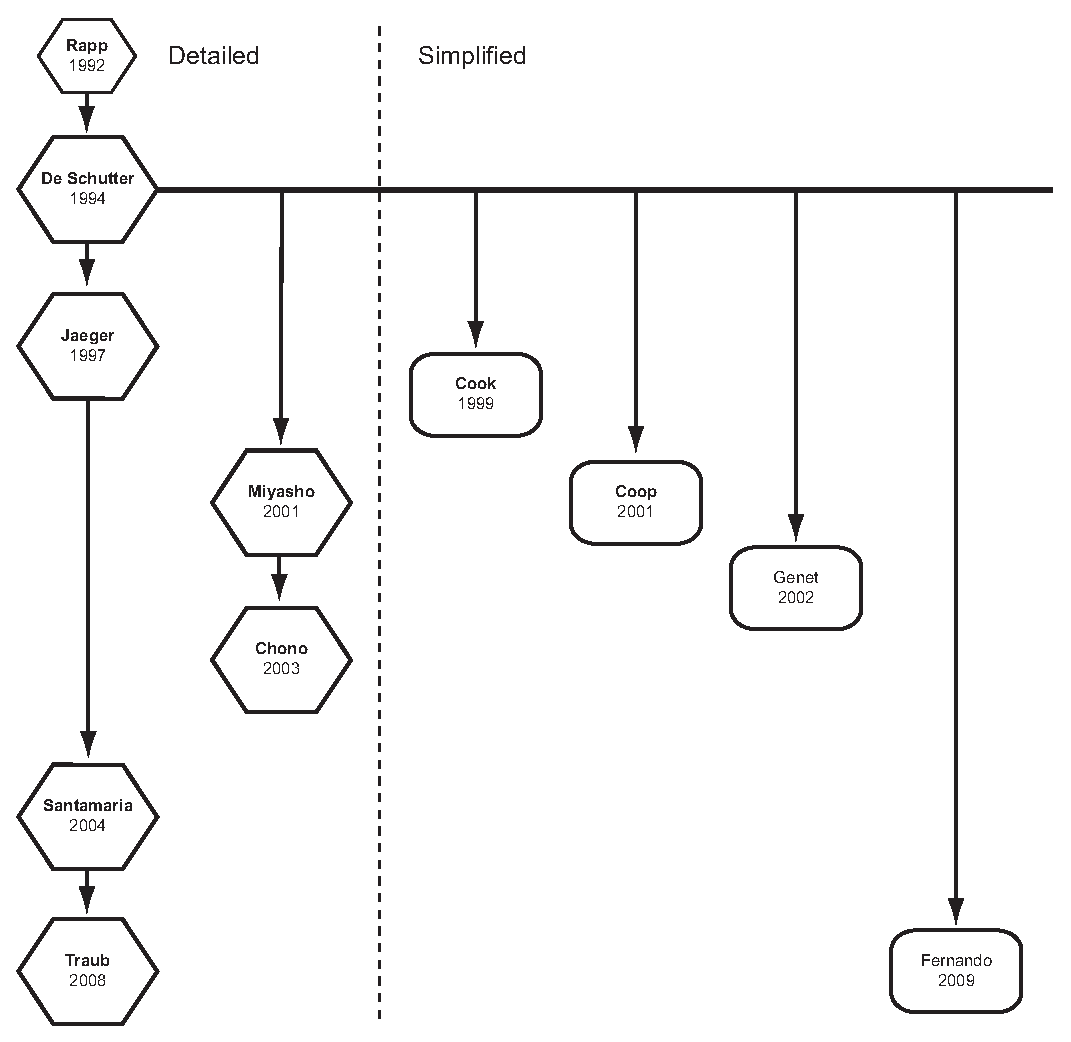
\includegraphics[scale=0.7]{figures/pc-lineage.eps}
\caption{{\bf Lineage system as attribution.} Hexagon indicates realistic multi-compartment model including dendritic morphology and Hodgkin-Huxley channel kinetics. Rectangle indicates model comprising simplified morphology and/or channel kinetics.}
  \label{fig:pcl-1}
\end{figure}

\bibliographystyle{plain}
\bibliography{../tex/bib/g3-refs.bib}

\end{document}
